\documentclass[aspectratio=169]{beamer}
\usepackage{beamerstyle}

% slides 7

\begin{document}

\begin{frame}
	\vspace{2cm}
	\begin{center}
		{\Huge\textbf{\textcolor{copenhagenred}{Slice Sampling}}}
		\vspace{1cm}

		\rule{4cm}{3pt}
		\vspace{2cm}
	\end{center}
\end{frame}

\begin{frame}{Slice Sampling}
	\begin{block}{What is Slice Sampling?}
		A ''black-box`` auxiliary variable Markov Chain Monte Carlo (MCMC) method that
		avoids the need to tune hyperparameters. Introduced by Neal (2003).
	\end{block}

	The idea of slice sampling. Suppose we wish to sample from a distribution for a
	variable, $x$, taking values in some subset of $R^n$ , whose density is proportional
	to some function $f (x)$. We can do this by sampling uniformly from the
	(n + 1)-dimensional region that lies under the plot of $f (x)$.
\end{frame}

\begin{frame}{Introduction}
	This idea can be
	formalized by introducing an auxiliary real variable, $y$, and defining a joint
	distribution over $x$ and $y$ that is uniform over the region
	$U = \{ (x,y):0 < y < f (x) \}$ below the curve or surface defined
	by $f (x)$. That is, the joint density for $(x,y)$ is

	\begin{equation*}
		p(x,y) = \frac{1}{Z} \begin{cases}
			1, & \text{if } 0 < y < f(x) \\
			0, & \text{otherwise}
		\end{cases}
	\end{equation*}

	where $Z = \int f(x)dx$. The marginal density for $x$ is then
	\begin{equation*}
		p(x) = \int_0^{f(x)} \frac{1}{Z} dy = \frac{f(x)}{Z}
	\end{equation*}
	which is the desired distribution. Thus, if we can sample from the joint
	distribution $p(x,y)$, we can obtain samples from the marginal distribution $p(x)$.
\end{frame}

\begin{frame}{Intuition Behind Slice Sampling}
	\begin{columns}[T]
		\begin{column}{0.48\textwidth}
			\textbf{Step 1: Vertical Slice}
			\begin{itemize}
				\item Given current position $x$
				\item Sample height $y \sim \text{Uniform}(0, \pi(x))$
				\item Defines horizontal ``slice'' at height $y$
			\end{itemize}
			\textbf{Step 2: Horizontal Slice}
			\begin{itemize}
				\item Sample new $x$ uniformly from slice
				\item $S = \{x : \pi(x) \geq y\}$
				\item Gives new sample from $\pi(x)$
			\end{itemize}		\end{column}
		\begin{column}{0.48\textwidth}
			\begin{center}
				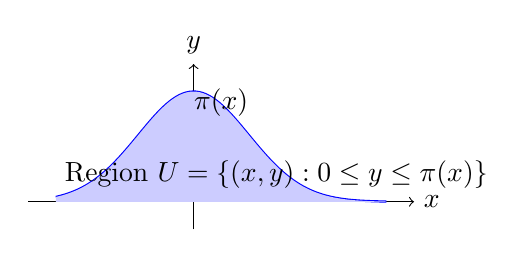
\begin{tikzpicture}[scale=0.7]
					\draw[->] (-3,0) -- (4,0) node[right] {$x$};
					\draw[->] (0,-0.5) -- (0,2.5) node[above] {$y$};
					\draw[thick,blue,domain=-2.5:3.5,smooth,samples=100] plot (\x,{2*exp(-(\x)^2/2)});
					\fill[blue!20,domain=-2.5:3.5,smooth,samples=100] plot (\x,{2*exp(-(\x)^2/2)}) -- (3.5,0) -- (-2.5,0) -- cycle;
					\node at (0.5,1.8) {$\pi(x)$};
					\node at (1.5,0.5) {Region $U = \{(x,y): 0 \leq y \leq \pi(x)\}$};
				\end{tikzpicture}
			\end{center}
			\textbf{Key Insight}:
				By alternating between sampling $y|x$ and $x|y$, we create a Markov chain that explores the space under $\pi(x)$ uniformly, with marginal distribution for $x$ being exactly $\pi(x)$
		\end{column}
	\end{columns}
\end{frame}

\begin{frame}{The Slice Sampling Algorithm}
	\begin{block}{Basic Algorithm}
		\textbf{Given:} Current state $x_t$, target distribution $\pi(x)$
	\end{block}
	\begin{block}{Algorithm}
		\begin{enumerate}
			\item \textbf{Sample auxiliary variable:} Draw $y \sim \text{Uniform}(0, \pi(x_t))$
			\item  \textbf{Find the slice:} Identify $S = \{x : \pi(x) \geq y\}$
			\item  \textbf{Sample from the slice:} Draw $x_{t+1} \sim \text{Uniform}(S)$
		\end{enumerate}
	\end{block}

	\vspace{0.3cm}
	\textbf{The Challenge: Finding and Sampling from $S$}

	In practice, finding $S = \{x : \pi(x) \geq y\}$ can be difficult!

	\highlighttext{\textbf{Key Idea: Leave Distribution Invariant}}
\end{frame}

\begin{frame}{How to sample from $S$}
	\begin{columns}[T]
		\begin{column}{0.48\textwidth}
			\begin{block}{The Stepping Out Procedure}
				\begin{enumerate}
					\item \textbf{Create initial interval:}
					\item $L = x_t - w \cdot U$, $R = L + w$, where $U \sim \text{Uniform}(0,1)$
					\item \textbf{Step out left:}
					\item While $\pi(L) \geq y$: $L = L - w$
					\item \textbf{Step out right:}
					\item While $\pi(R) \geq y$: $R = R + w$
				\end{enumerate}
			\end{block}
		\end{column}
		\begin{column}{0.48\textwidth}
			\begin{block}{The Shrinking Procedure}
				\begin{enumerate}
					\item \textbf{Sample and shrink:}
					\item Loop: $x' \sim \text{Uniform}(L, R)$
					\item If $\pi(x') \geq y$: accept $x_{t+1} = x'$
					\item Else: shrink $[L,R]$ by setting $L = x'$ or $R = x'$
				\end{enumerate}
			\end{block}
		\end{column}
	\end{columns}

	\textbf{Adaptive Nature}: The algorithm automatically adapts to the local scale of $\pi(x)$. Wide regions are explored with large steps, narrow regions with small steps.
	Alternative procedures exist for sampling from $S$ e.g., doubling.
\end{frame}


% \begin{frame}{Why $w$ is Not a Critical Tuning Parameter}

% 	\begin{block}{The Width Parameter $w$: Efficiency vs. Correctness}
% 		Yes, $w$ IS technically a tuning parameter, BUT...
% 	\end{block}

% 	\begin{columns}[T]
% 		\begin{column}{0.48\textwidth}
% 			\textbf{Traditional MCMC (e.g., RW-Metropolis)}
% 			\begin{itemize}
% 				\item \textbf{Poor tuning $\rightarrow$ Poor mixing}
% 				\item $\sigma$ too small $\rightarrow$ Tiny steps, stuck
% 				\item $\sigma$ too large $\rightarrow$ High rejection
% 				\item Can take exponentially long
% 				\item \highlighttext{Affects correctness in finite time}
% 			\end{itemize}
% 		\end{column}
% 		\begin{column}{0.48\textwidth}
% 			\textbf{Slice Sampling with $w$}
% 			\begin{itemize}
% 				\item \textbf{Poor $w$ $\rightarrow$ More computation}
% 				\item $w$ too small $\rightarrow$ Many step-outs
% 				\item $w$ too large $\rightarrow$ More shrinking
% 				\item Always finds correct slice
% 				\item \highlighttext{Only affects efficiency}
% 			\end{itemize}
% 		\end{column}
% 	\end{columns}
% \end{frame}

% \begin{frame}{Why $w$ is Not a Critical Tuning Parameter}
% 	\textbf{Why $w$ is Robust: The Self-Correcting Mechanism}

% 	\begin{columns}[T]
% 		\begin{column}{0.48\textwidth}
% 			\textbf{Case 1: $w \ll$ typical slice width}
% 			\begin{itemize}
% 				\item Initial $[L, R]$ doesn't cover slice
% 				\item Stepping-out expands it
% 				\item $\checkmark$ Still finds correct slice!
% 			\end{itemize}
% 		\end{column}
% 		\begin{column}{0.48\textwidth}
% 			\textbf{Case 2: $w \gg$ typical slice width}
% 			\begin{itemize}
% 				\item Initial $[L, R]$ too wide
% 				\item Shrinking contracts it
% 				\item $\checkmark$ Still samples correctly!
% 			\end{itemize}
% 		\end{column}
% 	\end{columns}

% 	\begin{block}{Mathematical Guarantee}
% 		For ANY $w > 0$:
% 		\begin{itemize}
% 			\item The stationary distribution is ALWAYS $\pi(x)$
% 			\item Detailed balance is satisfied
% 			\item Convergence is guaranteed
% 		\end{itemize}
% 	\end{block}

% 	\begin{alertblock}{Key Distinction}
% 		In slice sampling, $w$ affects ``how many function evaluations per sample'' not ``whether we get correct samples''
% 	\end{alertblock}
% \end{frame}

\begin{frame}{Why Slice Sampling Converges}

	\textbf{Formal Convergence Properties}

	\begin{block}{1. Detailed Balance}
		Let $T(x'|x)$ be the transition kernel. We need: $\pi(x) \cdot T(x'|x) = \pi(x') \cdot T(x|x')$
	\end{block}

	\textbf{Proof sketch:}
	\begin{itemize}
		\item Given $x$, sample $y \sim \text{Uniform}(0, \pi(x))$
		\item Probability density of moving from $x$ to $x'$:
		      $$T(x'|x) = \int_0^{\min(\pi(x),\pi(x'))} \frac{1}{\pi(x)} \cdot \frac{1}{|S_y|} dy$$
		      where $|S_y|$ is the length of slice $\{z : \pi(z) \geq y\}$
		\item This is symmetric: $T(x'|x) = T(x|x')$ $\Rightarrow$ detailed balance holds
	\end{itemize}
\end{frame}

\begin{frame}{Convergence - Continued}

	\begin{block}{2. Irreducibility}
		For any $x, x'$ where $\pi(x) > 0$ and $\pi(x') > 0$:
		$$P(x \to x') \geq \int_0^{\min(\pi(x),\pi(x'))} \frac{1}{\pi(x)} \cdot P(x' \text{ sampled from } S_y) dy > 0$$
	\end{block}

	\begin{block}{3. Aperiodicity}
		$P(x \to x) > 0$ (can stay at current state) $\Rightarrow$ period = 1
	\end{block}

	\begin{alertblock}{Ergodic Theorem}
		Since the chain is irreducible, aperiodic, with stationary distribution $\pi(x)$:
		$$\lim_{n\to\infty} \|P(X_n \in \cdot | X_0 = x_0) - \pi(\cdot)\|_{TV} = 0$$
	\end{alertblock}
\end{frame}


% \begin{frame}{Convergence: Additional Mathematical Details}

% 	\begin{block}{Detailed Balance - Complete Argument}
% 		Consider augmented state space $(x, y)$ with invariant distribution:
% 		$$\pi^*(x, y) = \frac{1}{Z} \cdot \indicator\{0 \leq y \leq \pi(x)\}$$
% 		where $Z = \int \pi(x)dx$ is the normalization constant.
% 	\end{block}

% 	\textbf{The Gibbs Sampler View}

% 	Slice sampling is a Gibbs sampler on the augmented space:
% 	\begin{itemize}
% 		\item \textbf{Step 1:} Sample $y | x \sim \text{Uniform}(0, \pi(x))$
% 		\item \textbf{Step 2:} Sample $x | y \sim \text{Uniform}(\{x : \pi(x) \geq y\})$
% 	\end{itemize}

% 	Each conditional distribution is correct:
% 	\begin{align}
% 		p(y|x) & = \frac{1}{\pi(x)} \cdot \indicator\{0 \leq y \leq \pi(x)\} \\
% 		p(x|y) & = \frac{1}{|S_y|} \cdot \indicator\{\pi(x) \geq y\}
% 	\end{align}

% 	\textbf{Why This Ensures Convergence:}
% 	\begin{enumerate}
% 		\item \textbf{Gibbs sampling preserves $\pi^*$:} Each conditional update leaves $\pi^*(x,y)$ invariant
% 		\item \textbf{Marginalization:} $\int_0^\infty \pi^*(x,y)dy = \pi(x)/Z \propto \pi(x)$
% 		\item \textbf{Detailed balance inherited:} Gibbs updates satisfy detailed balance by construction
% 	\end{enumerate}

% 	\begin{block}{Geometric Ergodicity (Bonus)}
% 		Under mild conditions ($\pi$ log-concave or exponential tails):
% 		$$\|P^n(x, \cdot) - \pi(\cdot)\|_{TV} \leq M(x)\rho^n, \quad \rho < 1$$
% 	\end{block}

% \end{frame}

\begin{frame}{Various topics}
	\begin{itemize}
		\item How to choose initial width $w$?
		\item Extensions to Multivariate Slice Sampling. Coordinate-wise: Apply one-dimensional slice sampling to
each $x_i$ in turn. (Gibbs sampling)
		\item Elliptical Slice Sampling for Gaussian priors (Murray et al., 2010)
	\end{itemize}
\end{frame}

\end{document}